\chapter{Lösungsansatz (Giulia)}
\section{Grundkonzept und verwendete Tools}
Grundbaustein der zu entwickelnden Anwendung ist ein Model-View-Controller Konzept (siehe Abbildung 4.1.). Es ermöglicht einen flexiblen Programmentwurf und reduziert die Entwicklungszeit hinsichtlich späteren Änderungen oder Erweiterungen. Unsere eigene nicht-relationale Datenbank, die mittels MongoDB \cite{mongodb} generiert wird, stellt hierbei das Model dar. MongoDB ist dokumentorientiert, sodass die von der NVD \cite{nvd} zur Verfügung gestellten JSON-Dateien einfach importiert werden können. Der View-Programmteil ist die GUI. Das Frontend verwendet hierfür JQuery, Bootstrap und JavaScript. Diese Tools ermöglichen zahlreiche Gestaltungsmöglichkeiten, um eine benutzerfreundliche, übersichtliche und intuitiv verständliche Oberfläche zu kreieren. Das Backend agiert als Controller und verbindet Model und View. Mithilfe der MongoDB können die NVD-Daten sehr schnell durchsucht und zurückgegeben werden.  \\
\begin{figure}[htb]
    \centering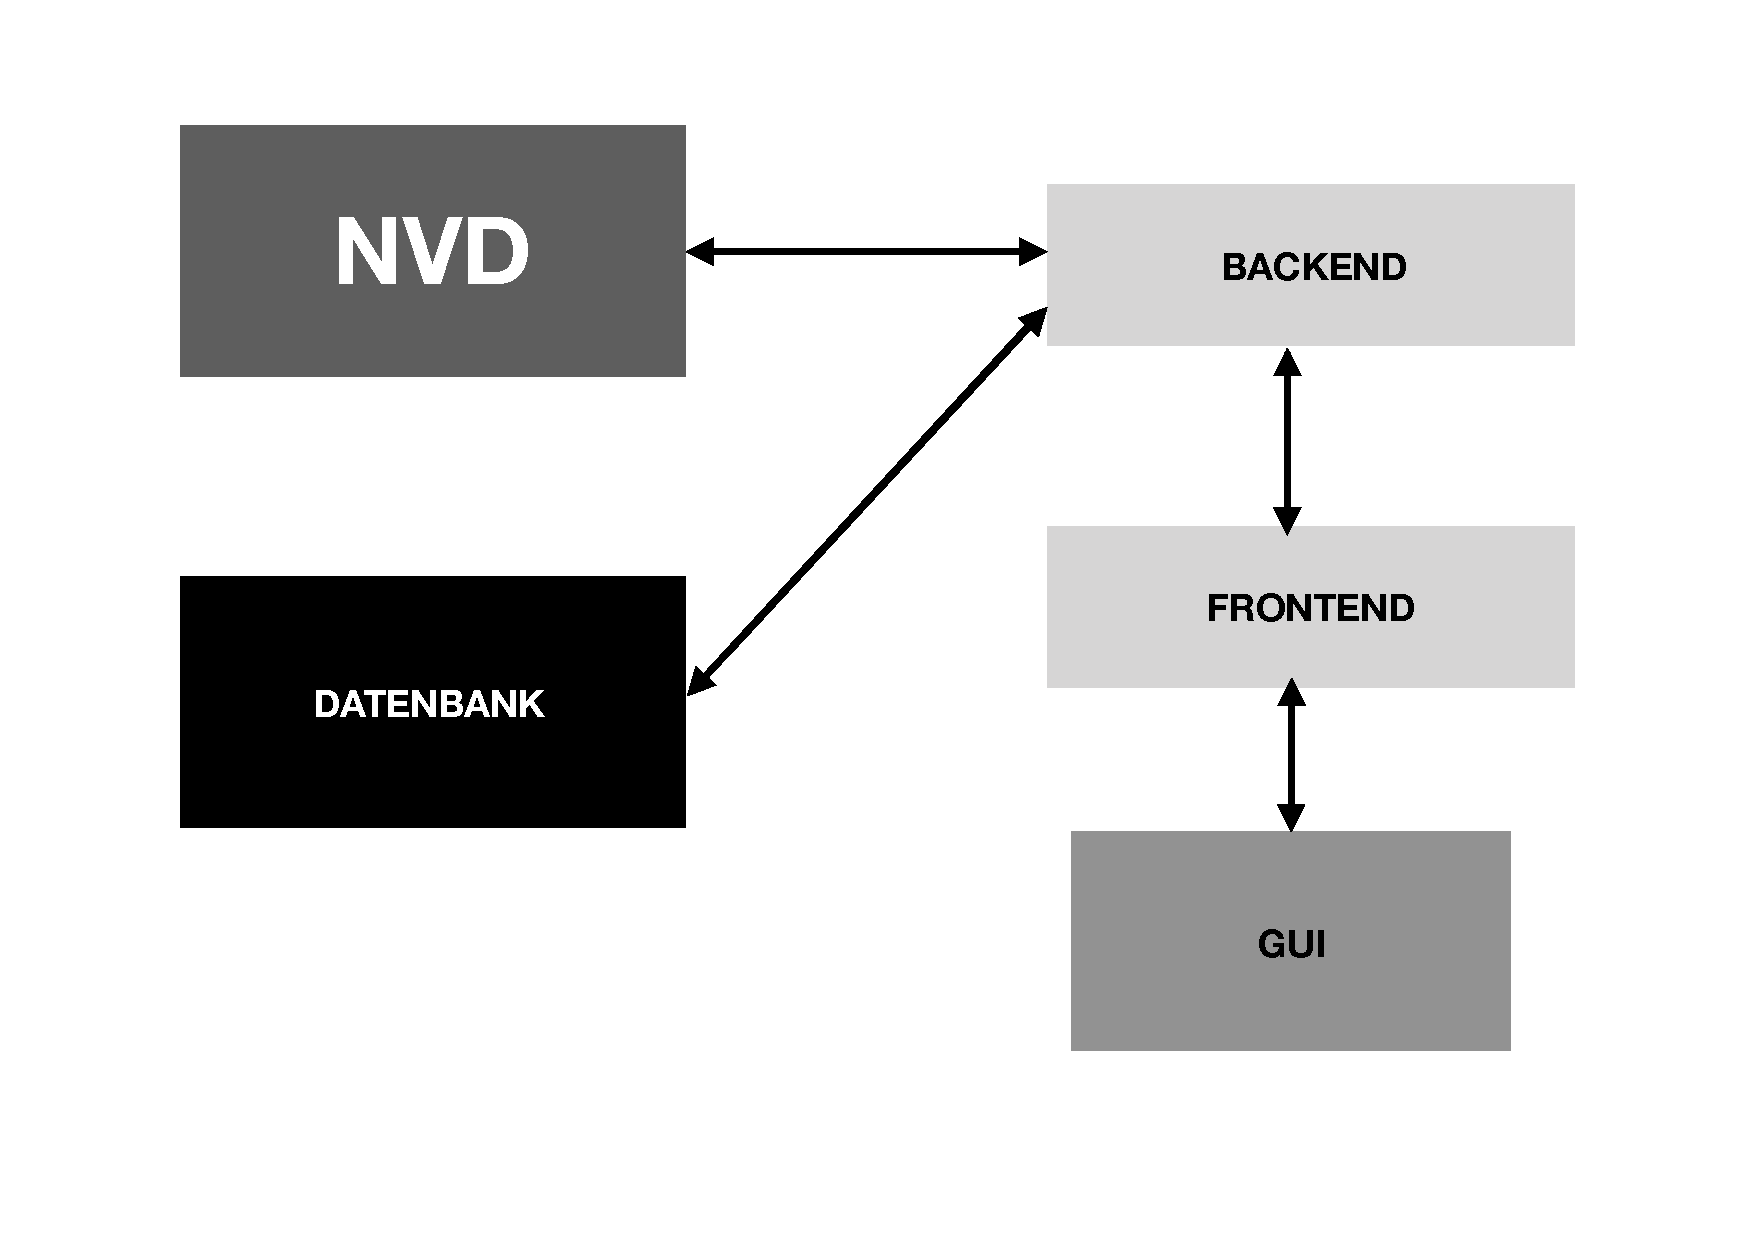
\includegraphics[scale=0.4]{figures/model.pdf}
    \caption{High-Level-Design: Model-View-Controller Modell}
\end{figure}
\\
Des Weiteren wird Spring MVC als Web Framework genutzt, mit dem schnell und einfach eine REST-konforme Webapplikation aufgesetzt werden kann und unter Anderem Dependency Injection ermöglicht wird \cite{johnson2004expert}. 
\section{Planung}
Die zur Verfügung stehenden 11 Wochen werden in 4 große Blöcke eingeteilt. 
Am Anfang des Projektes steht eine Woche, die ganz dem Brainstorming und der Reuqirementanalyse gewidmet ist. Hierbei sollen mögliche Frameworks und Tools, und mögliche Herangehensweisen in Betracht gezogen werden. Daraufhin folgt eine weitere Woche, die der Konzeption und der Entwicklung eines genauen Entwurfs dienen. Eine gute und detaillierte Planung von Back- und Frontend soll eine reibungslose Implementierung ermöglichen und Verzögerungen im weiteren Verlauf des Projekts verhindern. Nun stehen einige Tage zur Einrichtung zur Verfügung. Aufgrund von vier verschiedenen Betriebssystemen ist es wichtig dafür zu sorgen, dass alle auf dem gleichen Stand sind und miteinander interagieren können, z.B. via Git. Die nächsten Wochen dienen der Erstellung eines ersten Prototyps mit einer lokale Datenbank, die mit NVD \cite{nvd} Daten gespeist wird und einer ersten einfache Suche. Wenn diese Grundfunktionalitäten stehen, geht es um die Fertigstellung von Back- und Frontend mittels CI und CD. 
\\
Zur Umsetzung und schnelleren Implementierung wird das Team in zwei Arbeitsgruppen unterteilt – ein Expertenteam für Front- und eins für Backend. Durch wöchentliche Meetings und eine regelmäßige Kommunikation via Slack und Telegram ist die Abstimmung und Synchronisierung der Schnittstellen problemlos. Die letzte Woche vor Abschluss des Projekts soll Zeit einräumen, die fertige GUI, die Suche und Feinheiten zu testen, und entsprechende Tests zu schreiben. \\\\
\begin{figure}[htb]
    \centering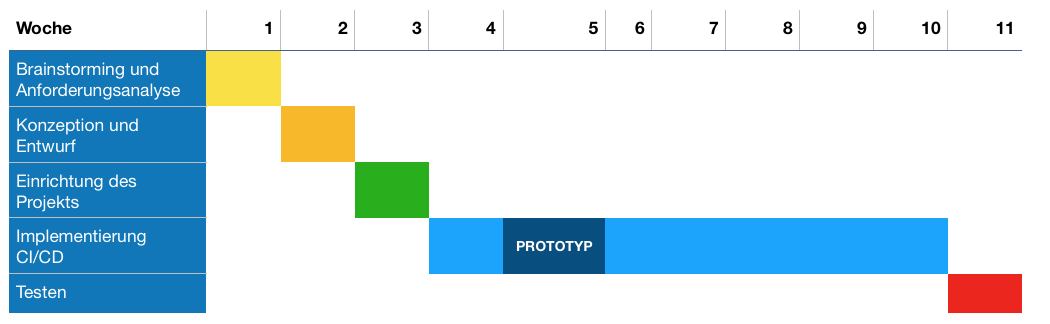
\includegraphics[scale=0.82]{figures/GANTT3}
    \caption{Gantt-Diagramm}
\end{figure}